\documentclass{article}
\usepackage[utf8]{inputenc}
\usepackage{listings}
\usepackage{geometry}
\usepackage{graphicx}

\graphicspath{.}
\title{COMP1204 Data management: Coursework 2}
\author{Kritagya Gurung}

\begin{document}

	
	\maketitle
	\begin{center}
		Student ID: 30220238
	\end{center}
	
	\newpage

	\section{The Relational Model}

	\subsection{EX1}
	
	\begin{center}
		\begin{tabular}{||c c | c c | c c ||} 
			\hline
			Attribute name & data type & Attribute name & data type & Attribute name & data type \\
			\hline
			Hotel ID & int & Overall rating & float & Avg. Price & int \\ 
			URL & string & Author & string & Content & string \\ 
			Date & string & No. Reader & int & No. Helpful & int \\ 
			Overall & int & Value & int & Rooms & int \\
			Location & int & Cleanliness & int & Check in/Front desk & int \\
			Service & int & Business service & int &  &  \\
			\hline
		\end{tabular}
	\end{center}
	Relation Schema: 
	\newline
	(R1)Review(Hotel ID, Overall rating, Avg. Price, URL, Author, Content, Date, No. Reader, No. Helpful, Overall, Value, Rooms, Location, Cleanliness, Check in/Front desk, Service, Business service).
	\newline
	The primary key consists of Hotel ID, Author and date. This is because all other attributes rely on the attributes mentioned and in order to write a review, you must have an author, the date that review was written on and what hotel the review is for.
		
	\subsection{EX2}
	\begin{math}
		\textrm{Hotel ID}
		\rightarrow
		\textrm{Overall rating, Avg. Price, URL}
	\end{math}
	\newline
	Hotel ID is the determinant for Overall rating, Avg. Price and URL. This is because each hotel has their own distinct properties.
	\newline
	\begin{math}
		\textrm{Author, Date}
		\rightarrow
	\end{math}
	Content, No. Reader, No. Helpful, Overall, Value, Rooms, Location, Cleanliness, Check in/Front desk, Service, Business service.
	\newline
	Author and Date should be the determinant for all other attributes since it is the author who decides the scores and the content of the review on a hotel. Additionally, the author must stay at the hotel thus date is used to show when the hotel was reviewed.
	\newline
	Candidate keys:
	\newline
	Hotel ID, Author, Date
	\subsection{EX3}
	\begin{center}
		\begin{tabular}{||c c | c c | c c ||} 
			\hline
			Attribute name & data type & Attribute name & data type & Attribute name & data type \\
			\hline
			Hotel ID & int & Overall rating & float & Avg. Price & int \\ 
			URL & string & Author & string & Content & string \\ 
			Date & string & No. Reader & int & No. Helpful & int \\ 
			Overall & int & Value & int & Rooms & int \\
			Location & int & Cleanliness & int & Check in/Front desk & int \\
			Service & int & Business service & int & User ID & int \\
			\hline
		\end{tabular}
	\end{center}
	Hotel(Hotel ID, Avg. Price, Date) \\
	Review(Hotel ID, User ID, Content, Date, No. Reader, No. Helpful, Overall, Value, Rooms, Location, Cleanliness, Check in/Front desk, Service, Business service) \\
	Author(User ID, Author) \\
	Primary Key : Hotel ID, User ID, Date \\
	Foreign Key : Hotel ID, User ID \\
	
	\section{Entity-Relationship Diagramming}
	
	\subsection{EX4}
	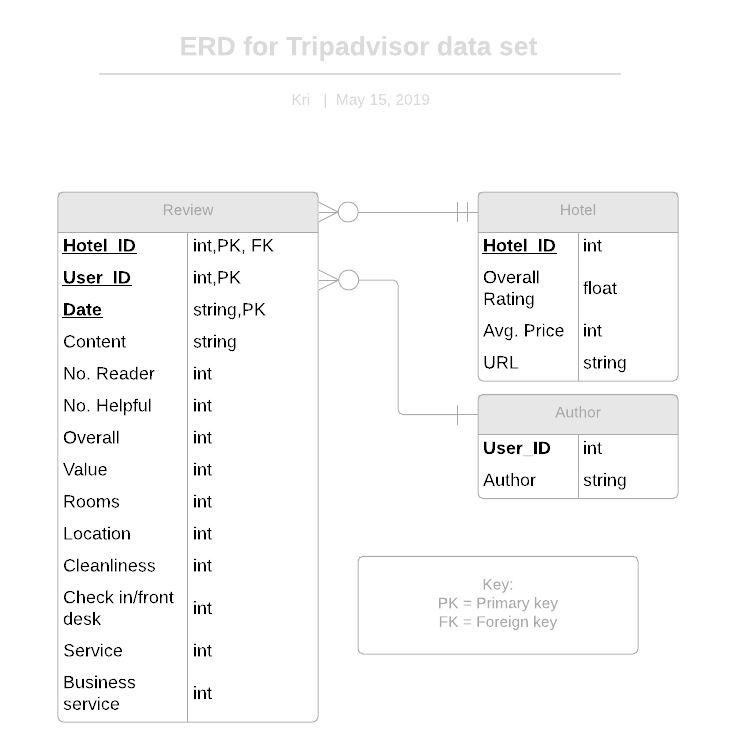
\includegraphics[width=10cm, height=10cm]{EX4_ERD_Tripadvisor.png}
	
	
	\section{Relational Algebra}
	
	\subsection{EX5}
	\begin{eqnarray}
	\sigma_{User ID = given ID}(Review)
	\end{eqnarray}
		
	\subsection{EX6}
	\begin{eqnarray}
	\sigma _{No. reviews given > 2}(_{User ID} \gamma _{count(User ID) \rightarrow No. reviews given}(Review)) \bowtie Author
	\end{eqnarray}
	
	\subsection{EX7}
	\begin{eqnarray}
		\sigma _{No. reviews recieved > 10}(_{Hotel ID} \gamma _{count(Hotel ID) \rightarrow No. reviews recieved}(Review))
	\end{eqnarray}
	
	\subsection{EX8}
	\begin{eqnarray}
	\sigma _{Average cleanliness \geq 4.5 \wedge Overall rating > 3}(_{Hotel ID} \gamma _{avg(Cleanliness) \rightarrow Average cleanliness}(Review) \bowtie (Hotel))
	\end{eqnarray}
	
	\section{SQL Queries}
	
	\subsection{EX9}
	
	\subsection{EX10}
	
	\subsection{EX11}
		
	\subsection{EX12}
	
	\subsection{EX13}
	
	\subsection{EX14}
	
	\section{Conclusions}
	
	\subsection{EX15}

\end{document}